\documentclass{tuna-report}
\usepackage{codespace}
\usepackage{caption}
\usepackage{subcaption}
\usepackage{wrapfig}
\usepackage{graphicx}
\usepackage{array}

% Sub-preambles
% https://github.com/MartinScharrer/standalone

% Side by side tables
\usepackage{geometry}
% \usepackage{xcolor}

% Encodings
\usepackage{gensymb,textcomp}

% Better tables
% Wide tables go to https://tex.stackexchange.com/q/332902
\usepackage{multicol,multirow,siunitx,tabularx}

% Better enum
\usepackage{enumitem}

% Graphics
\usepackage{caption,float}

% Allow setting >max< width of figure
% 'export' allows adjustbox keys in \includegraphics
% For demonstration purposes, remove in production
\usepackage[export]{adjustbox}

% For demonstration purposes, remove in production
\usepackage{mwe}

% Configurations
\newcounter{memberrowno}
\setcounter{memberrowno}{0}
\setcounter{tocdepth}{5}
\reportlayout%

% Override (some) default values
\ocoursename{Compulsory Elective Subject: Data Analysis in High Dimensions}
% \ocoursedetails{Data Analysis in High Dimensions}
\title{Hierarchical Cluster Analysis: Movie Genres Preferences}
\oadvisor{Prof. Christina Andersson}

% Custom commands
\newcommand*\mean[1]{\bar{#1}}

\begin{document}
\coverpage%

\section*{Member list \& Workload}
\noindent Our team has 4 members and we together decide to split the total workload into proper parts equally. Each member is responsible for the work as below: 

\vspace {2pt}
\begin{center}
  \begin{tabular}{>{\stepcounter{memberrowno}\thememberrowno}llcc}
    \toprule
    \multicolumn{1}{c}{\textbf{No.}} & \textbf{Full name} & \textbf{ID} & \textbf{Percentage of work} \\
    \midrule
    & Vu Hoang Tuan Anh     & 18812     & 100\%                       \\
    & Tran Kim Hoan         & 18810     & 100\%                       \\
    & Ba Nguyen Quoc Anh    & 17965     & 100\%                      \\
    & Nguyen Hoang Hai Nam  & 17035     & 100\%                     \\
    \bottomrule
  \end{tabular}
\end{center} 
\vspace {2pt}

\begin{itemize}
    \item \textbf{Vu Hoang Tuan Anh} (ID: 18812)
        \begin{itemize}
            \item[-] Collecting and preparing data
            \item[-] Applying hierarchical cluster model with dummy variables
            \item[-] Analysising results, plotting dendrogram and histogram, distribution diagram
            \item[-] Using Gap Statistics method to find the optimal number of clusters
            \item[-] Writing the report (4. Hierarchical clustering with Dummy variables)
        \end{itemize}
        
    \item \textbf{Tran Kim Hoan} (ID: 18810)
        \begin{itemize}
            \item[-] Conducting the survey
            \item[-] Collecting and preparing data
            \item[-] Applying hierarchical cluster model with dummy variables
            \item[-] Analysising results, plotting dendrogram, histogram
            \item[-] Writing and finalizing the report (3. Data)
        \end{itemize}
        
    \item \textbf{Ba Nguyen Quoc Anh} (ID: 17965)
        \begin{itemize}
            \item[-] Collecting data
            \item[-] Applying hierarchical clustering model with Gower's distance
            \item[-] Analysising results, plotting dendrogram, histogram
            \item[-] Writing the report (5. Hierarchical clustering with mixed-type variables + 6. Conclusion)
        \end{itemize}

    \item \textbf{Nguyen Hoang Hai Nam} (ID: 17035)
        \begin{itemize}
            \item[-] Conducting the survey
            \item[-] Collecting data
            \item[-] Applying hierarchical cluster model with dummy variables
            \item[-] Writing the report (1. Project Objective + 2. Overview of Hierarchical clustering methodology)
        \end{itemize}
\end{itemize}



\newpage
\newpage

\tableofcontents


\section{Project Objective}

%\begin{itemize}

   % \item Briefly summarize the purpose of the analysis and its abstracts. Highlight the implications for the recommend system.
    
   % \item Provide an introduction to the report, explaining the context and goals of the hierarchical cluster analysis.
%\end{itemize}

%\begin{enumerate}
  %  \item We would like to group together users with similar viewing patterns in order to recommend similar content (genres). By asking different questions about age, genre, hobbies, we can collect data and conclude some insights.

   %  \item The data will be collect and analysis by using R software 

    
 
  
      We would like to group together users with similar viewing patterns in order to recommend similar content (genres). By asking different questions about age, genre, hobbies, we can collect data and conclude some insights.

    

    

    
   % \end{itemize}

%\end{enumerate}

\section {Overview of Hierarchical clustering methodology}
Hierarchical clustering is an algorithm that groups similar objects into clusters. The clusters are distinct from each other, and the objects within each cluster are broadly similar to each other.

Hierarchical clustering is an unsupervised learning technique. This means that a model does not have to be trained, and there is no need for a "target" variable.

There are two common categories of Hierarchical clustering, agglomerative and divisive. 

\begin{itemize}
    \item Agglomerative clustering starts in it individual clusters, then merges pair of clusters and continuing until all clusters have been merge in one huge clusters.

        \begin{figure}[H]
            \centering
            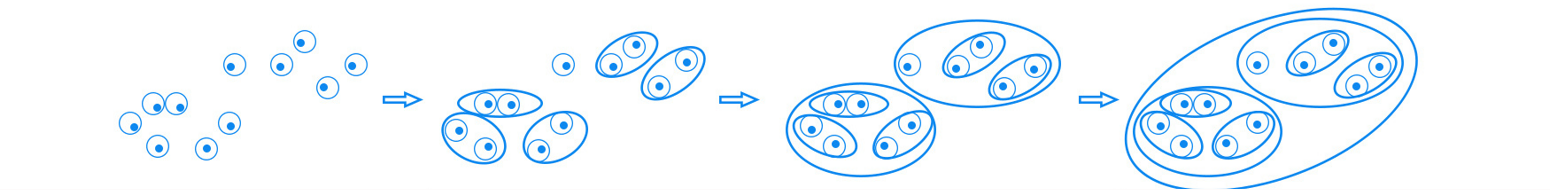
\includegraphics[scale=0.4]{graphics/overview/Agglomerative.png}
            \caption{Agglomerative clustering}
        \end{figure}

    \item Divisive clustering is the inverse approach of agglomerative clustering which starts in one cluster then splits into smaller cluster base on their difference.

        \begin{figure}[H]
            \centering
            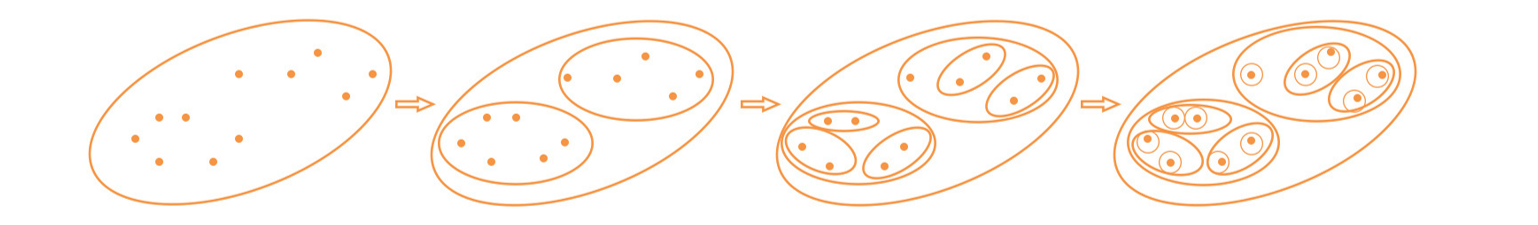
\includegraphics[scale=0.4]{graphics/overview/Diversive.png}
            \caption{Divisive clustering}
        \end{figure}
\end{itemize}
In our project, we only focus on agglomerative clustering.




The method of hierarchical clustering starts by treating each data point as a separate cluster and then iteratively combines the closest clusters until a stopping criterion is reached. The clusters are visually represented in a hierarchical tree called a dendrogram. 

\begin{figure}[H]
     \centering
     \begin{subfigure}[b]{0.3\textwidth}
         \centering
         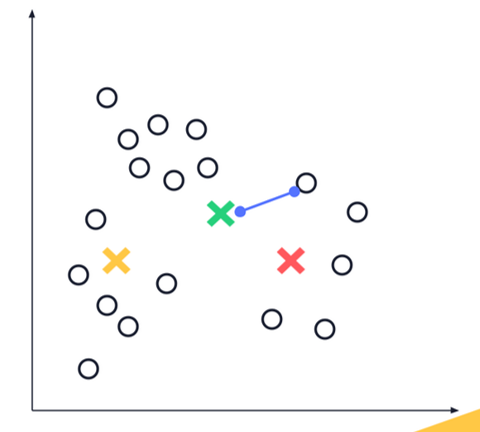
\includegraphics[width=\textwidth]{graphics/overview/FIndDistance.png}
         \caption{Finding points distances}
         % \label{fig:audau1701}
     \end{subfigure}
     \hfill
     \begin{subfigure}[b]{0.3\textwidth}
         \centering
         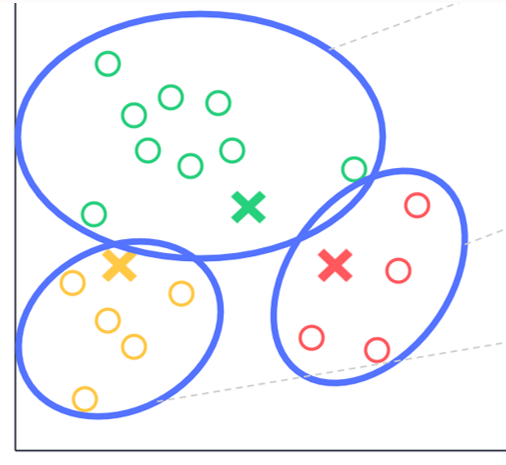
\includegraphics[width=\textwidth]{graphics/overview/Grouping.png}
         \caption{Grouping}
     \end{subfigure}
     \hfill
     \begin{subfigure}[b]{0.3\textwidth}
         \centering
         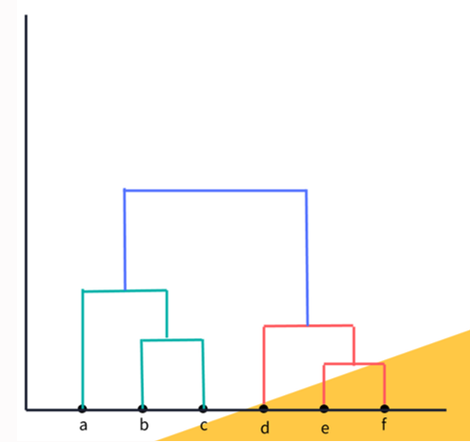
\includegraphics[width=\textwidth]{graphics/overview/Termination.png}
         \caption{Termination}
     \end{subfigure}
        \caption{Hierarchical clustering steps}
\end{figure}

\begin{enumerate}
    \item \textbf{Finding points distances:} Calculate the distance between each point of observation. There are various mathematical algorithms to apply: "euclidean", "maximum", "manhattan", "canberra", "binary", "minkowski"

    \item \textbf{Grouping points (clustering)} Calculate the distance between each cluster. There are various mathematical algorithms to apply:"Ward", "single", "complete", "average", "mcquitty", "median", "centroid". After that, choose the optimal number of clusters. 

    \item \textbf{Termination} Plotting the final dendrogram and starting the analysis process based on attributes of each cluster.
\end{enumerate}


% \section {Overview of Hierarchical clustering methodology}
% Hierarchical clustering is an algorithm that groups similar objects into clusters. The clusters are distinct from each other, and the objects within each cluster are broadly similar to each other.

% Hierarchical clustering is an unsupervised learning technique. This means that a model does not have to be trained, and there is no need for a "target" variable.

% There are two common categories of Hierarchical clustering, agglomerative and diversive. Agglomerative clustering starts in it individual clusters, then merges pair of clusters and continuing until all clusters have been merge in one huge clusters. Diversive clustering is the inverse approach of agglomerative clustering which starts in one cluster then splits into smaller cluster base on their difference. In our project, we only focus on allgomerative clustering  


% The method of hierarchical clustering starts by treating each data point as a separate cluster and then iteratively combines the closest clusters until a stopping criterion is reached. The clusters are visually represented in a hierarchical tree called a dendrogram. 
\section{Data}
According to the objective of our project, we require data for our analysis. Our data is derived from our online survey conducted over a week. All collected data is accessible only to authorized research team members.
    \subsection{Attributes Identification and Selection}
    Initially, we brainstorm and identify key attributes which will be included in our analysis such as user demographics, user behavior and user preferences. After discussing their relevance and potential impact on the user’s movie genre preferences, we eventually determine seven key attributes essential for our analysis: age, gender, working/learning area, preferred film genre, factor influencing genre choice, frequency of movie watching, source of film viewing.
            
        \subsection{Data Collection}
        \begin{itemize}
            \item \textbf{Step 1: Create a survey}\\
            We create a survey titled ‘Movie Genre Preferences’ to collect data via Google Forms. In the form, we focus on seven key attributes that we determined before. (as discussed in Section 2.1).
            \begin{figure}[H]
                \centering
                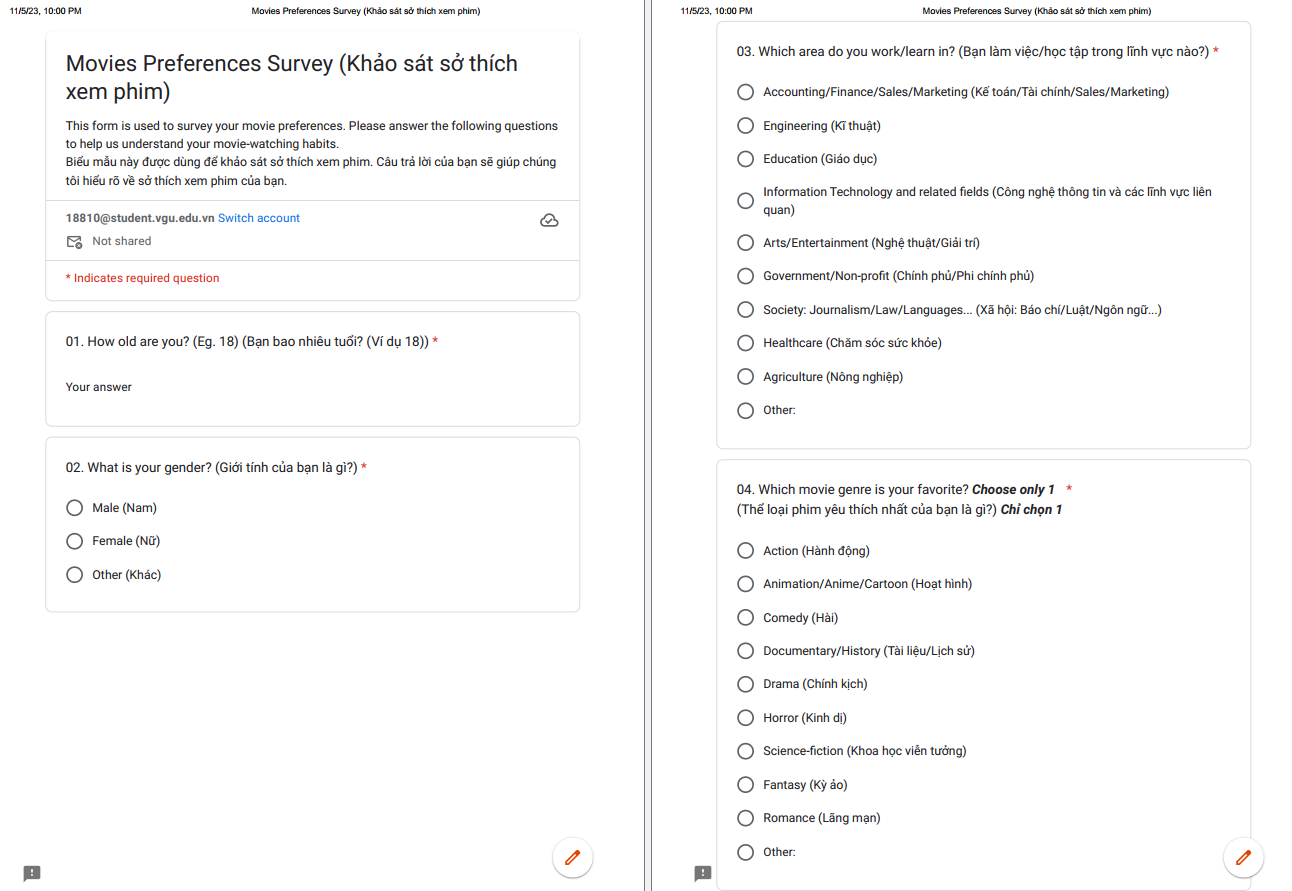
\includegraphics[scale=0.5]{graphics/data/Survey1.png}
                \caption{Movie genre preferences survey image (1)}
            \end{figure}
            
            \begin{figure}[H]
                \centering
                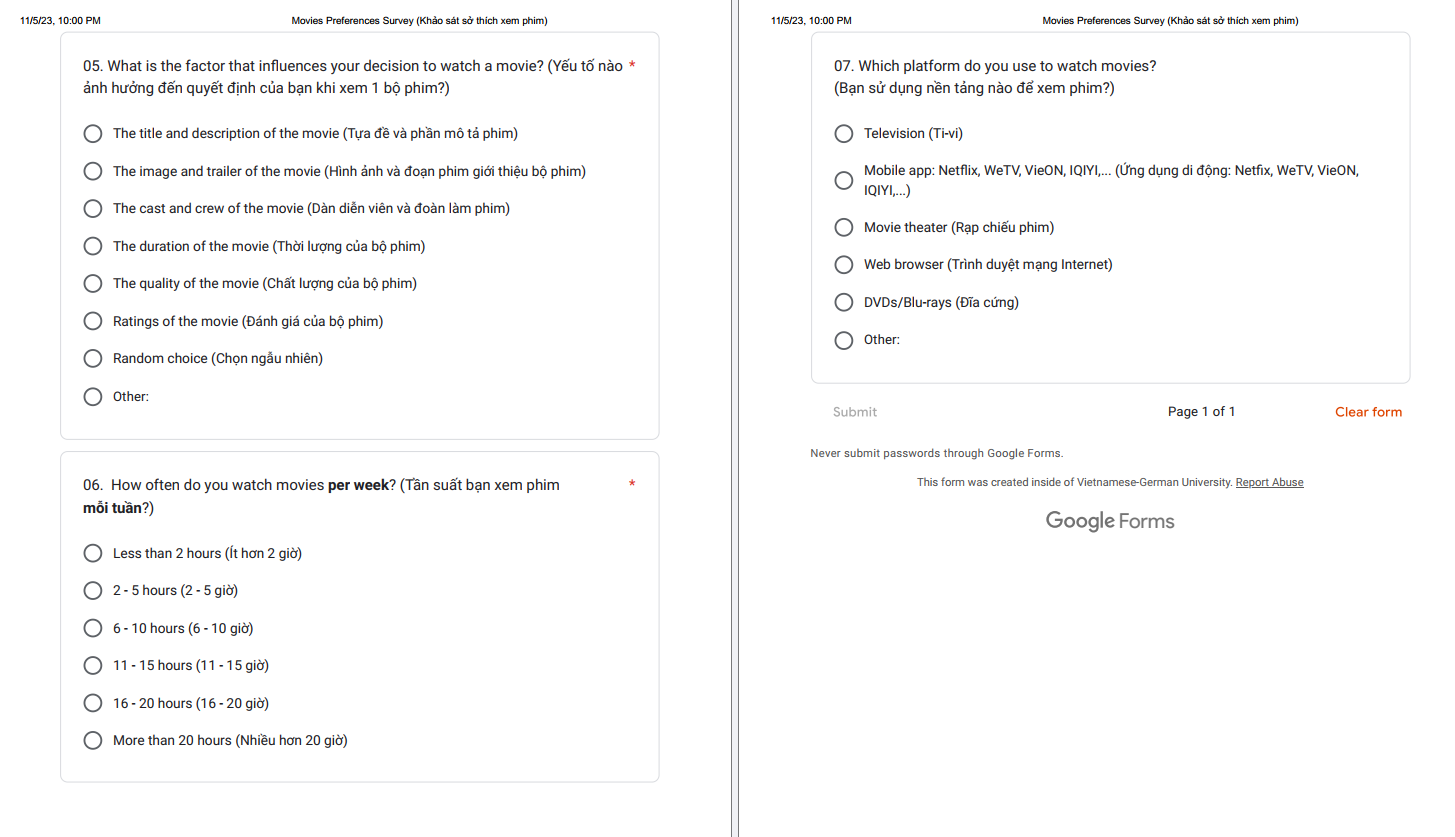
\includegraphics[scale=0.5]{graphics/data/Survey2.png}
                \caption{Movie genre preferences survey image (2)}
            \end{figure}
            
            \item \textbf{Step 2: Publish survey and receive responses}\\
            After completing the form, we distribute it to individuals, specifically targeting those aged 16 and above. Subsequently, we received a total of 118 responses from the survey. \\
            Here is an image of the responses list:
                \begin{figure}[H]
                    \centering
                    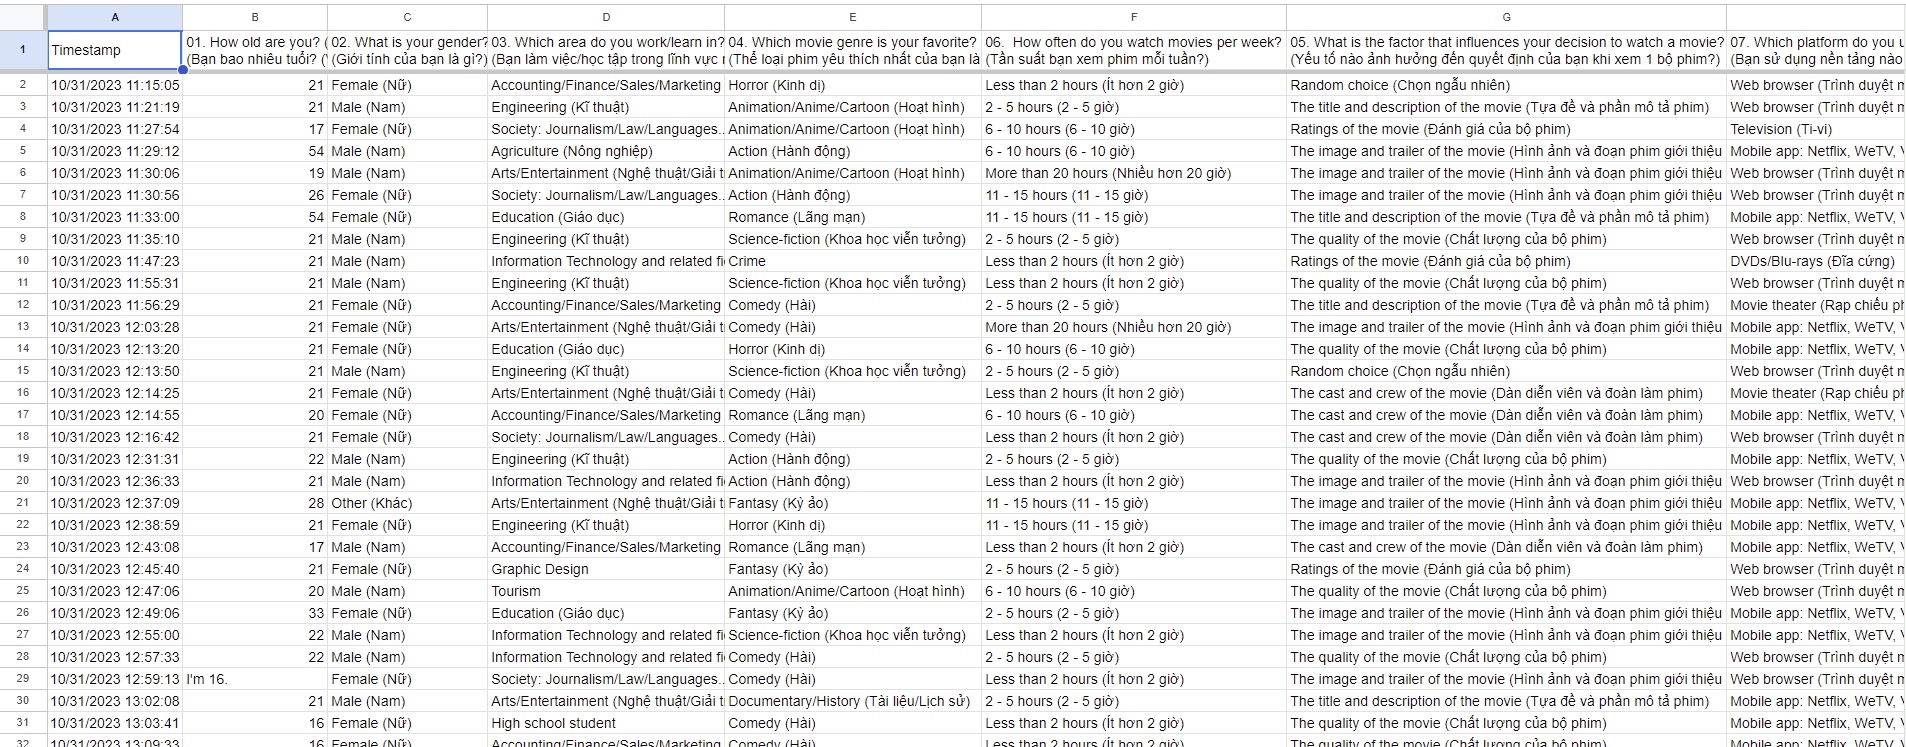
\includegraphics[scale=0.4]{graphics/data/dataResponses1.png}
                    \caption{Image of the responses list}
                \end{figure}
        \end{itemize}
        
    \subsection{Data Preparation}
   This process is crucial in minimizing the potential for errors and inaccuracies that may arise during our data processing stage. By ensuring the data is accurately prepared and processed, we can enhance the reliability and validity of our analysis.
    
    With a dataset of 118 responses, we come to the first crucial step for our data analysis: cleaning data.
                \begin{itemize}
                    \item In terms of attributes, we convert them from question format to word/phrase format:
                        \begin{figure}[H]
                            \centering
                            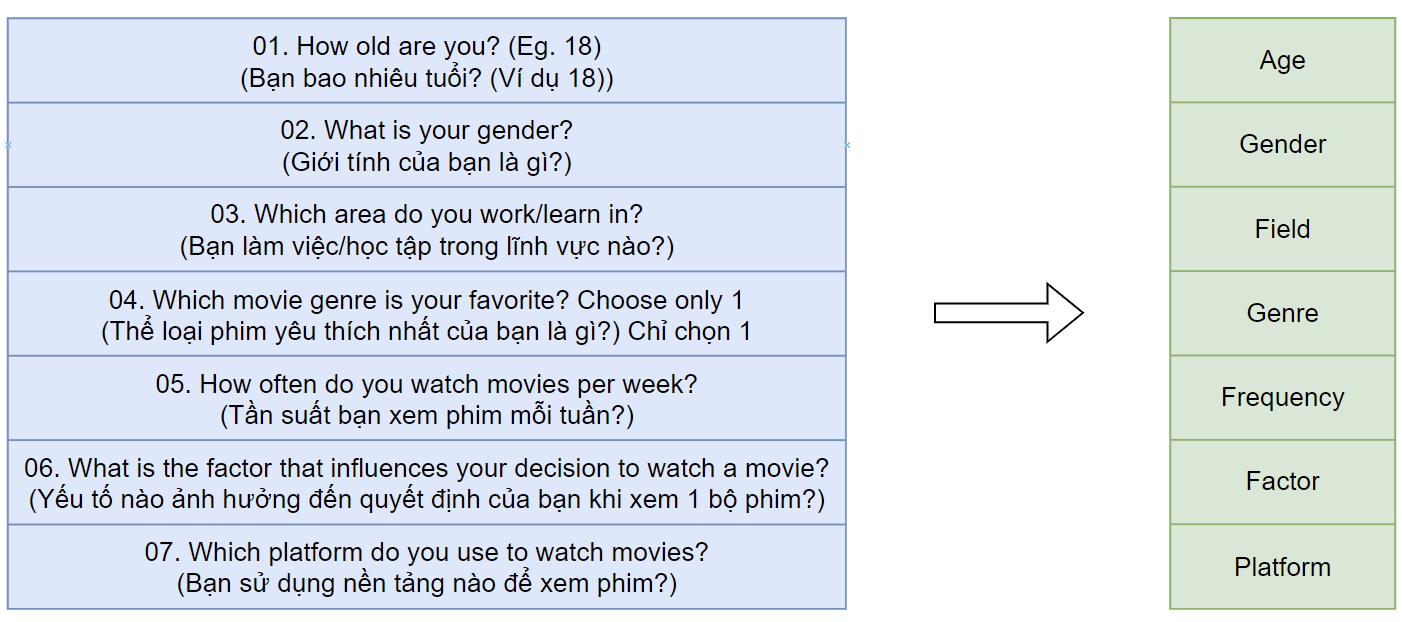
\includegraphics[scale=0.45]{graphics/data/questiontophrase1.png}
                            \caption{Image of attributes before and after}
                        \end{figure}
                    
                    \item We also substitute long words/phrases with shorter ones:
                         \begin{figure}[H]
                            \centering
                            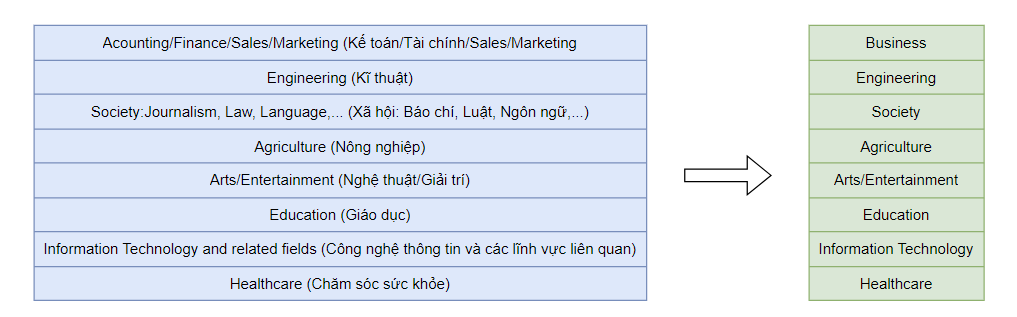
\includegraphics[scale=0.65]{graphics/data/substi.png}
                            \caption{Image of the data before and after substitution}
                        \end{figure}

                    \item Regarding working/learning area,  we decided to combine "real estate" as a part of "business":
                        \begin{figure}[H]
                            \centering
                            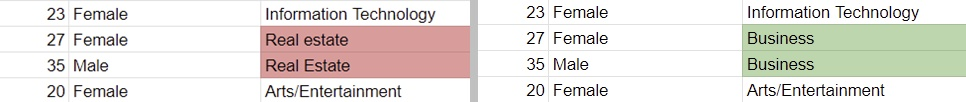
\includegraphics[scale=0.5]{graphics/data/realestate_business.jpg}
                            \caption{Image of the data before and after combination}
                        \end{figure}
                    
                    \item We adjust responses that are not in the correct format into our anticipated format:
                        \begin{figure}[H]
                            \centering
                            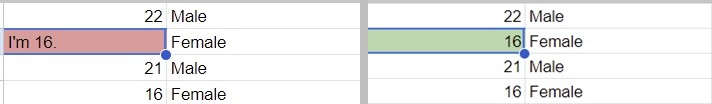
\includegraphics[scale=0.5]{graphics/data/Wrongformat3.jpg}
                            \caption{Image of the data before and after}
                        \end{figure}
                        
                    \item We remove responses that deviate from our expected range of values:
                        \begin{figure}[H]
                            \centering
                            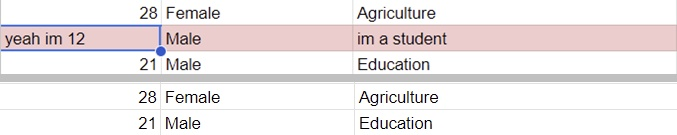
\includegraphics[scale=0.6]{graphics/data/eliminate3.jpg}
                            \caption{Image of the data example before and after elimination}
                        \end{figure} 

                    \item The entry “housewife” does not correspond to a specific work or learning area. Therefore, we exclude it from our dataset:
                        \begin{figure}[H]
                            \centering
                            
\includegraphics[scale=0.75]{graphics/data/housewife.png}
                            \caption{Image of the entry "housewife"}
                        \end{figure} 
                    After the data cleaning process, we obtain the final dataset. This dataset has the correct format, concise words/phrases, and values within an appropriate range for all attributes, making it suitable for our analysis.
                    \begin{figure}[H]
                        \centering
                        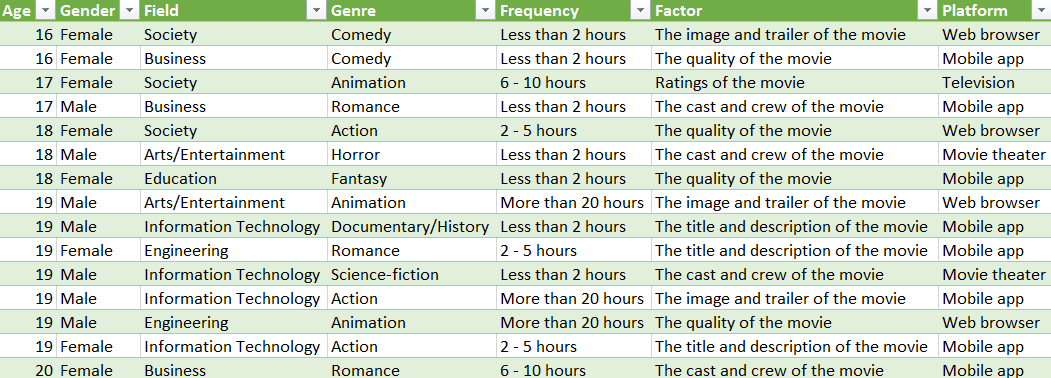
\includegraphics[scale=0.65]{graphics/data/finaldata.png}
                        \caption{Image of the final data after data cleaning process}
                    \end{figure} 
            In the next step, we apply the hierarchical clustering method to our final dataset, using dummy variables and mixed-type variables.
                \end{itemize}
\section{Hierarchical clustering with Dummy variables}

% \begin{itemize}
%     \item Present the results of the hierarchical clustering analysis. This include dendrogram plots, cluster sizes, and statistics.
%     \item Describe the number of clusters or groups identified and their characteristics.
%     \item Provide profiles or descriptions of the clusters. Discuss what makes each cluster unique in terms of viewing patterns and behavior.\\
%     Include statistics or visualizations that highlight the key features of each cluster.
%     \item Recommendations for the Recommender System.\\
%     Explain how the clustering results can be applied to the recommender system.\\
%     Describe how content recommendations can be tailored to each cluster's preferences.\\
%     Discuss any challenges or considerations in implementing these recommendations.
%     \item Evaluation of the Recommender System\\
%     Discuss how the clustering-based recommender system was evaluated, including metrics such as accuracy, user satisfaction, or engagement.\\
%     Present the results of the evaluation and any improvements made based on feedback.
%     \item Pros and Cons of methods using to analysis
% \end{itemize}



\subsection{Problem}
    Regarding the objective of the project, users with similar viewing patterns need to be grouped together in a cluster, and in the previous section, we know that the dataset consists of both numerical and categorical data. Especially, it is impossible to calculate the distance between any 2 entries of the data frame by applying mathematical algorithms (Euclidean, Manhattan, Canberra, etc) directly since all variables are not numerical. To handle this situation, an encode is needed to convert variables from nominal to numerical type. (The conversion from ordinal variables to numerical variables is redundant since ordinal variables could be labeled with levels and then be scaled to behavior as numerical variables). That encoding is called \textbf{\textit{Dummy variables}}, and this section will discuss the implementation of dummy variables for hierarchical clustering.

\subsection{Dummy variables}

        \begin{itemize}
            \item \textbf{\underline{Definition:}} A Dummy (or Indicator) variable is an artificial variable created to represent a categorical variable with two or more distinct categories or levels.

            \item \textbf{\underline{Usage:}} With dummy variables, all nominal variables could be converted to numerical. Hence, it is possible to apply mathematical algorithms to start the analysis process.

            \item \textbf{\underline{Example:}} A nominal variable named "Genre" always takes one of 3 values "Action", "Comedy", and "Fantasy". After converting it into the dummy variable: 
            \begin{itemize}
                \item[-] If the value of the variable is "Action", the indicator for "Genre.Action" attribute will be 1, and other attributes are 0's.
                \item[-] If the value of the variable is "Comedy", the indicator for "Genre.Comedy" attribute will be 1, and other attributes are 0's.
                \item[-] If the value of the variable is "Fantasy", the indicators for all attributes are 0's.
            \end{itemize}
            
        \end{itemize}

\begin{table}[h]
\centering
 \begin{subtable}[b]{0.45\linewidth}
    \centering
      \begin{tabular}{|l|}
        \hline
          \cellcolor{blue!25}Genre \\
        \hline
         Action \\
         \hline
         Comedy \\
         \hline
          Fantasy \\
          \hline
       \end{tabular}
       \caption{Original "Genre" variable}
    \end{subtable}%
 \begin{subtable}[b]{0.45\linewidth}
        \centering
        \begin{tabular}{|l|c|c|}
            \hline
             & Genre.Action & Genre.Comedy \\
            \hline
            Action & 1 & 0 \\
            \hline
            Comedy & 0 & 1 \\
            \hline
            Fantasy & 0 & 0 \\
            \hline
        \end{tabular}
        \caption{"Genre" Dummy variable}
    \end{subtable}
    \caption{Using Dummy variables}
\end{table}

$\rightarrow $ A variable which has a total of $n$ different values will have new $n - 1$ attributes after converting to a dummy variable, and the last value has the indicators for all attributes are 0's.


\subsection{Applying the Hierarchical clustering model}

    \begin{itemize}
        \item In this section, R programming language is used as the main language to implement the hierarchical clustering model.

         \item Dependencies (List of packages used):

                 \begingroup
                    \setlength{\tabcolsep}{10pt} % Default value: 6pt
                    \renewcommand{\arraystretch}{1.2} % Default value: 1
                    \begin{tabular}{ | l | l |  l |} % l for left, c for center
                      \hline
                    \textbf{Package name} & \textbf{Description} & \textbf{Version} \\
                      \hline 
                    base & The R Base Package & $\ge 4.3.2$\\
                      \hline
                    cluster & Finding Groups in Data &  $\ge 2.1.4 $ \\
                      \hline
                    factoextra & clustering visualization &  $\ge 1.0.7 $ \\
                      \hline
                    gplots & plotting data, dendrogram &  $\ge 3.1.3 $ \\
                      \hline
                    ggplot2 & draw distribution graph &  $\ge 3.4.4 $ \\
                      \hline
                      
                    \end{tabular}
                \endgroup
         
    \end{itemize}

   
    \vspace{2mm}
    
    (Source code link: \url{https://github.com/vhtuananh020402/Group4_Data_analysis/blob/main/dummy_canberra_ward.r})
    
    \vspace{2mm}

    To start applying the hierarchical clustering model, first, the dataset is imported and stored as a data frame in R. The function \textbf{\textit{na.omit()}} is necessary for omitting the missing value of the imported data frame. 
    \begin{code}{R}
        # Read the data frame
        df <- read.csv("data/clean_data_v2.csv")
        
        # Omit the NA values of the data frame
        df <- na.omit(df)
    \end{code}

    Then, we standardize (scale) the "Age" (numerical) variables. Since the "Frequency" variable is ordinal, it first needs to be ordered and labeled with levels, then converted to a numerical variable using \textbf{\textit{as.numeric()}} function. After that, the "Frequency" (numerical) variable is scaled.

    \begin{code}{R}
        # Standardize the Age variable
        df$Age_std <- scale(df$Age)
        
        # Standardize the Frequency variable
        df$Frequency <- factor(
              df$Frequency, 
              order = TRUE,
              levels = c("Less than 2 hours", "2 - 5 hours", "6 - 10 hours", "11 - 15 hours", "16 - 20 hours", "More than 20 hours"))
        df$Frequency_numeric <- as.numeric(factor(df$Frequency))
        df$Frequency_std <- scale(df$Frequency_numeric)
    \end{code}

    The function \textbf{\textit{model.matrix()}} is used to create a data frame matrix consisting of all numerical variables (all nominal variables "Genre", "Field", "Factor", "Gender", "Platform" are converted to dummy variables)
    
    \begin{code}{R}
        # Turn the nominal variables into dummy variables
        df_dummy <- model.matrix(~ Age_std + Genre + Frequency_std + Field + Factor + Gender + Platform, data = df)
    \end{code}

    Here we use Canberra algorithms to calculate the points distance and Ward's method to calculate the clusters distance. Then we can visualize the hierarchical clusters by using the function \textbf{\textit{plot()}} to plot a dendrogram.
    
    \begin{code}{R}
        # Calculate the points distance
        point_dist <- dist(df_dummy, method = "canberra")      # Using Canberra distance
        
        # Hierarchical cluster analysis on the data frame
        hc <- hclust(point_dist, method = "ward.D")            # Using Ward's method
        
        # Plot the dendrogram
        dend <- as.dendrogram(hc)
        plot(dend)
    \end{code}

    \begin{figure}[H]
        \centering
        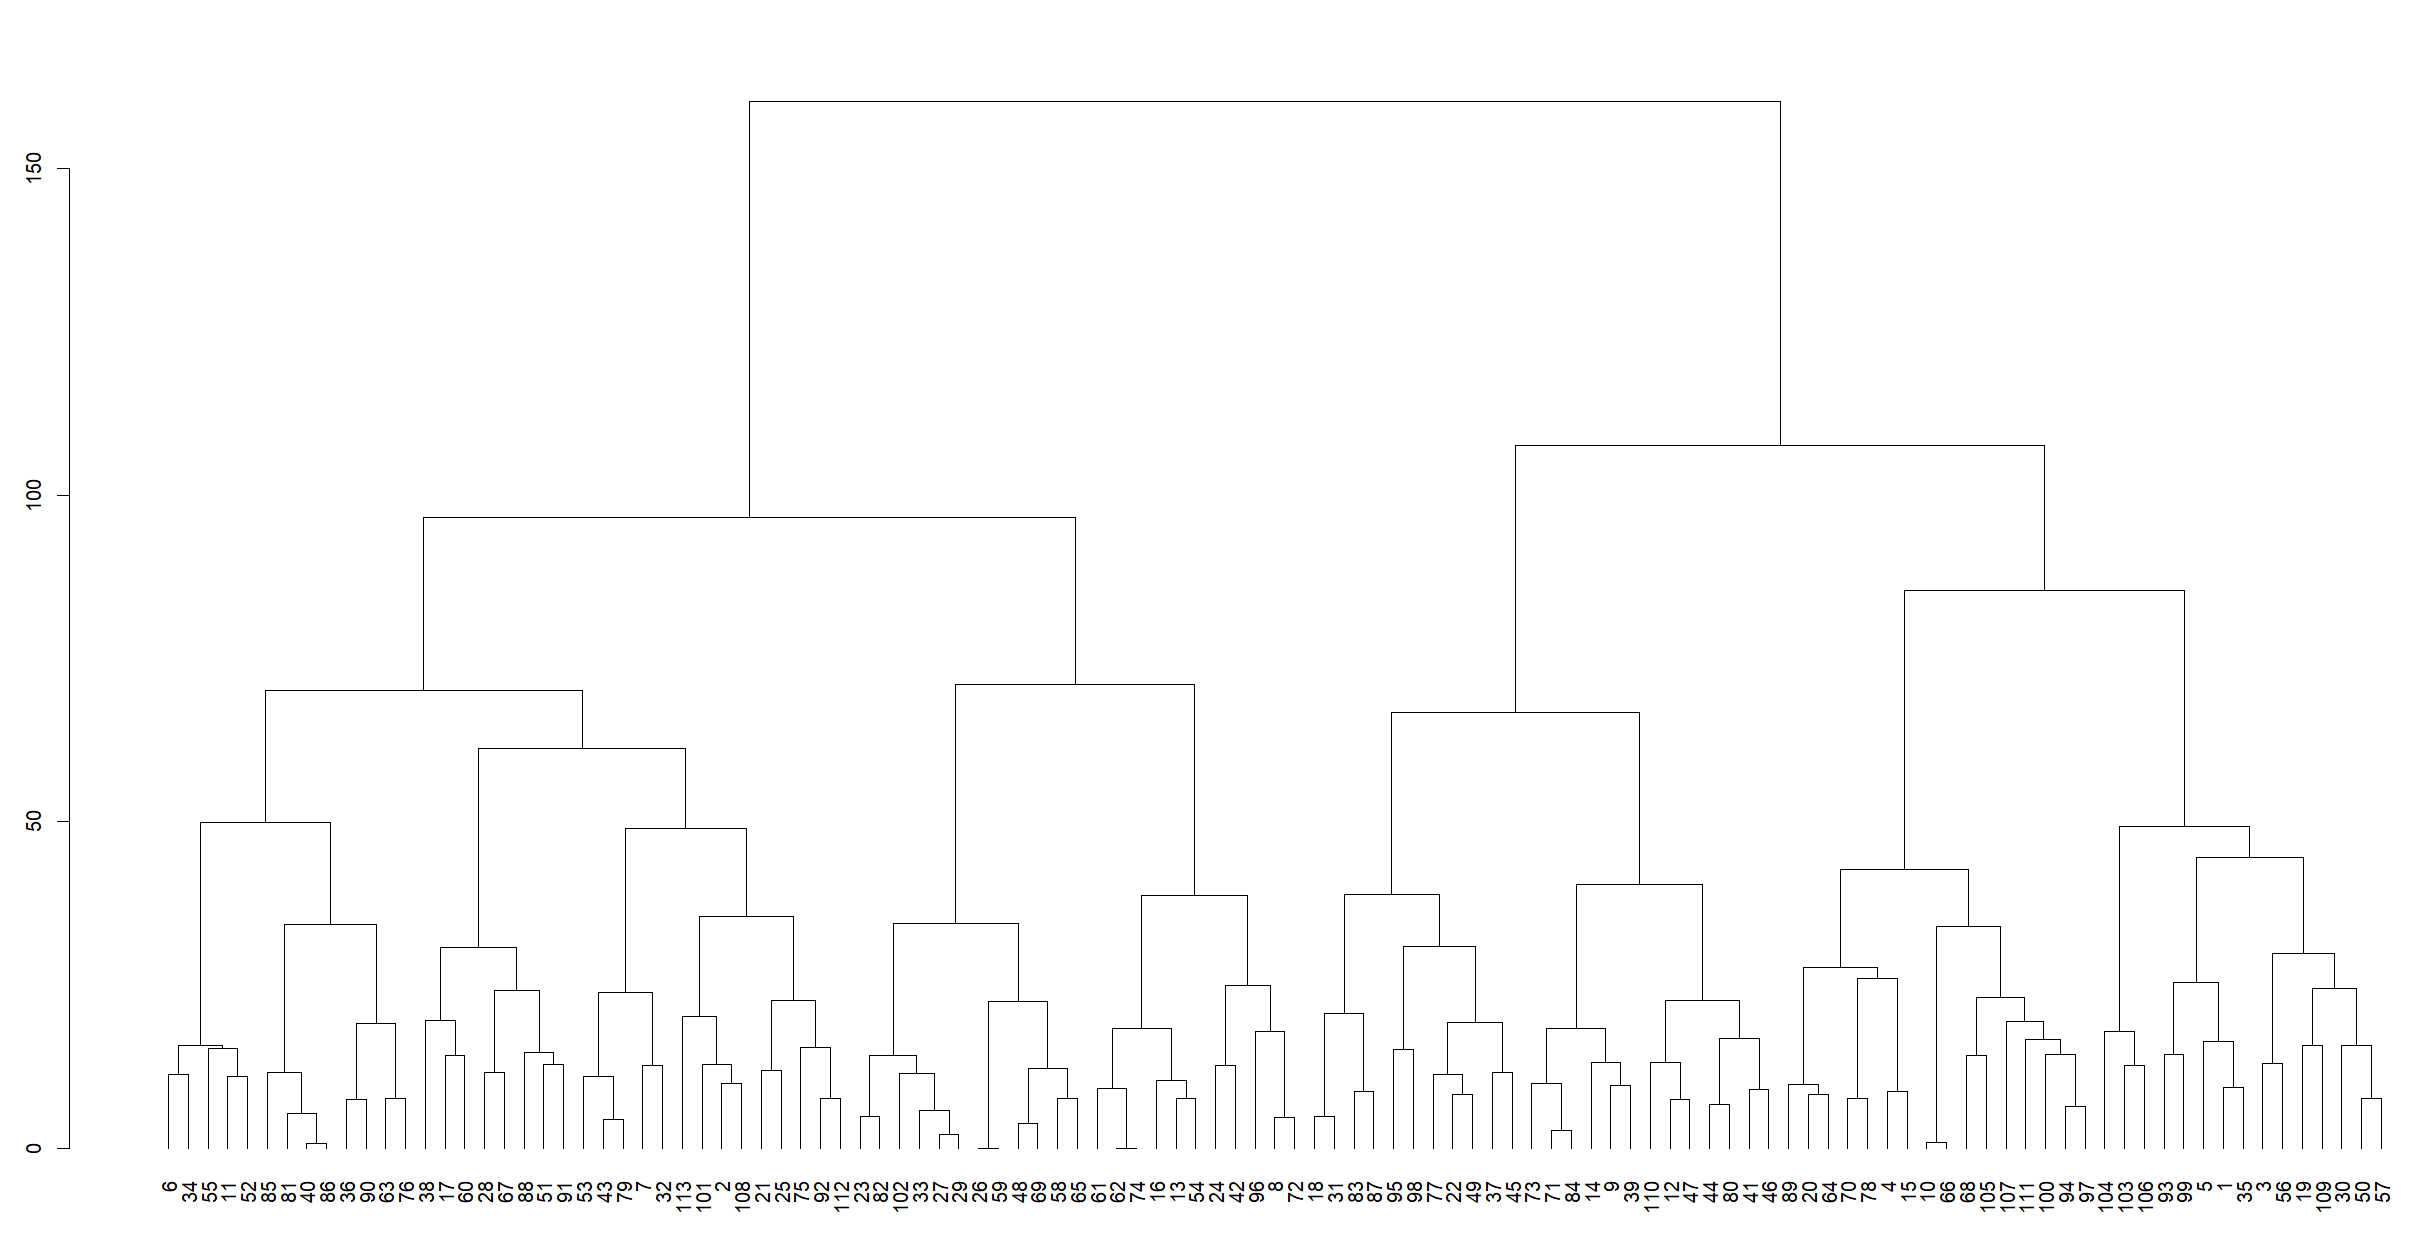
\includegraphics[scale=0.3]{graphics/dummy/dendrogram/dendrogram1.png}
        \caption{Dendrogram visualization }
    \end{figure} 

\subsection{Finding the optimal number of clusters}
 After dendrogram visualization, as can be clearly seen that there are many possible numbers of clusters to choose from for analysis. Each different number of clusters will bring different outcomes, thus we need an exact optimal number of clusters, and there are some methods that help us to find it, \textbf{Gap Statistics} is one of the most well-known and easily understandable methods to find the optimal number of clusters, so this section will focus on it.
 
    \subsubsection{Gap statistics method}

    \begin{itemize}
        \item This approach can be applied to any clustering method.

        \item The estimate of the optimal clusters will be the value that maximizes the gap statistic. This means that the clustering structure is far away from the random uniform distribution of points.

        \item R code implementation:
    \end{itemize}

    \begin{code}{R}
        # ======= Gap statistic method to find the optimal number of cluster  =======
        # Calculate Within-Cluster Dispersion (WCD) for the original data
        wss <- sum(hc$height)
        
        # Generate Random Data for Comparison
        set.seed(123)   # Set seed for reproducibility
        B <- 100        # Number of random datasets
        random_datasets <- lapply(1:B, function(i) matrix(runif(length(df_dummy)), ncol = ncol(df_dummy)))
        
        # Cluster the Random Data
        random_hcs <- lapply(random_datasets, function(random_data) {
          dist_matrix <- dist(random_data, method = dist_method[4])
          hclust(dist_matrix, method = hc_method[1])
        })
        
        # Calculate Within-Cluster Dispersion for Random Data
        wss_random <- sapply(random_hcs, function(random_hc) sum(random_hc$height))
        
        # Calculate Gap Statistic    
        gap <- (log(wss_random) - log(wss)) + mean(log(wss_random) - log(wss))
        
        # Determine the Optimal Number of Clusters
        num_clusters <- 1 : 10 # Desired number of cluster domain
        gap <- gap[1:length(num_clusters)]   
        x_labels <- seq(1, length(num_clusters))
        
        plot(num_clusters, gap, xlab = "Number of Clusters", ylab = "Gap Statistic", 
             main = "Gap Statistic Plot", type = "b")
        
        # Customize x-axis labels
        axis(1, at = x_labels, labels = num_clusters)
        abline(v = 8, col = "red", lty = 2)
    \end{code}


    \begin{figure}[H]
        \centering
        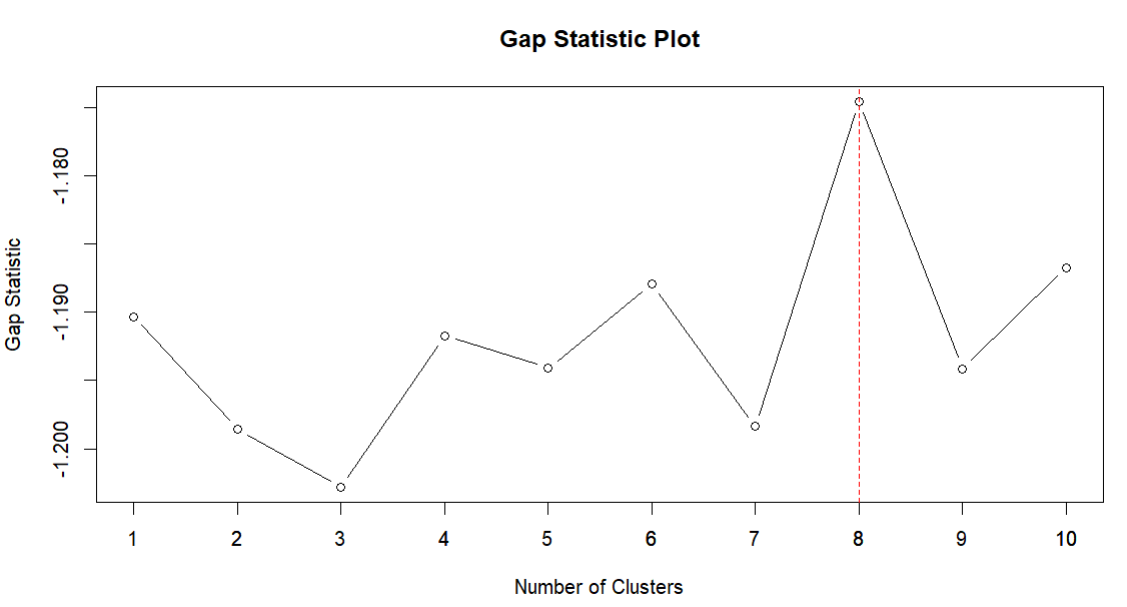
\includegraphics[scale=0.53]{graphics/dummy/gapStatistics/gapStatistics.png}
        \caption{Gap Statistics diagram}
    \end{figure}

    $\rightarrow$ From the above Gap Statistics diagram (range $1 : 10$), the highest point which indicates the optimal number of clusters for the dendrogram is 8. Hence, we chose the number 8 for the number of clusters for the dendrogram. 
    

\subsection{Result}
    \subsubsection{Dendrogram}


    \begin{code}{R}
        # Draw the rectangle around each cluster in k clusters
        k <- 8
        rect.hclust(hc, k, border = 2:8)
    \end{code}
    
    Here is the final dendrogram with 8 clusters, each cluster has a rectangle around it. The observations in each cluster have a close relationship, which will be discussed right after this dendrogram.

    \begin{figure}[H]
        \centering
            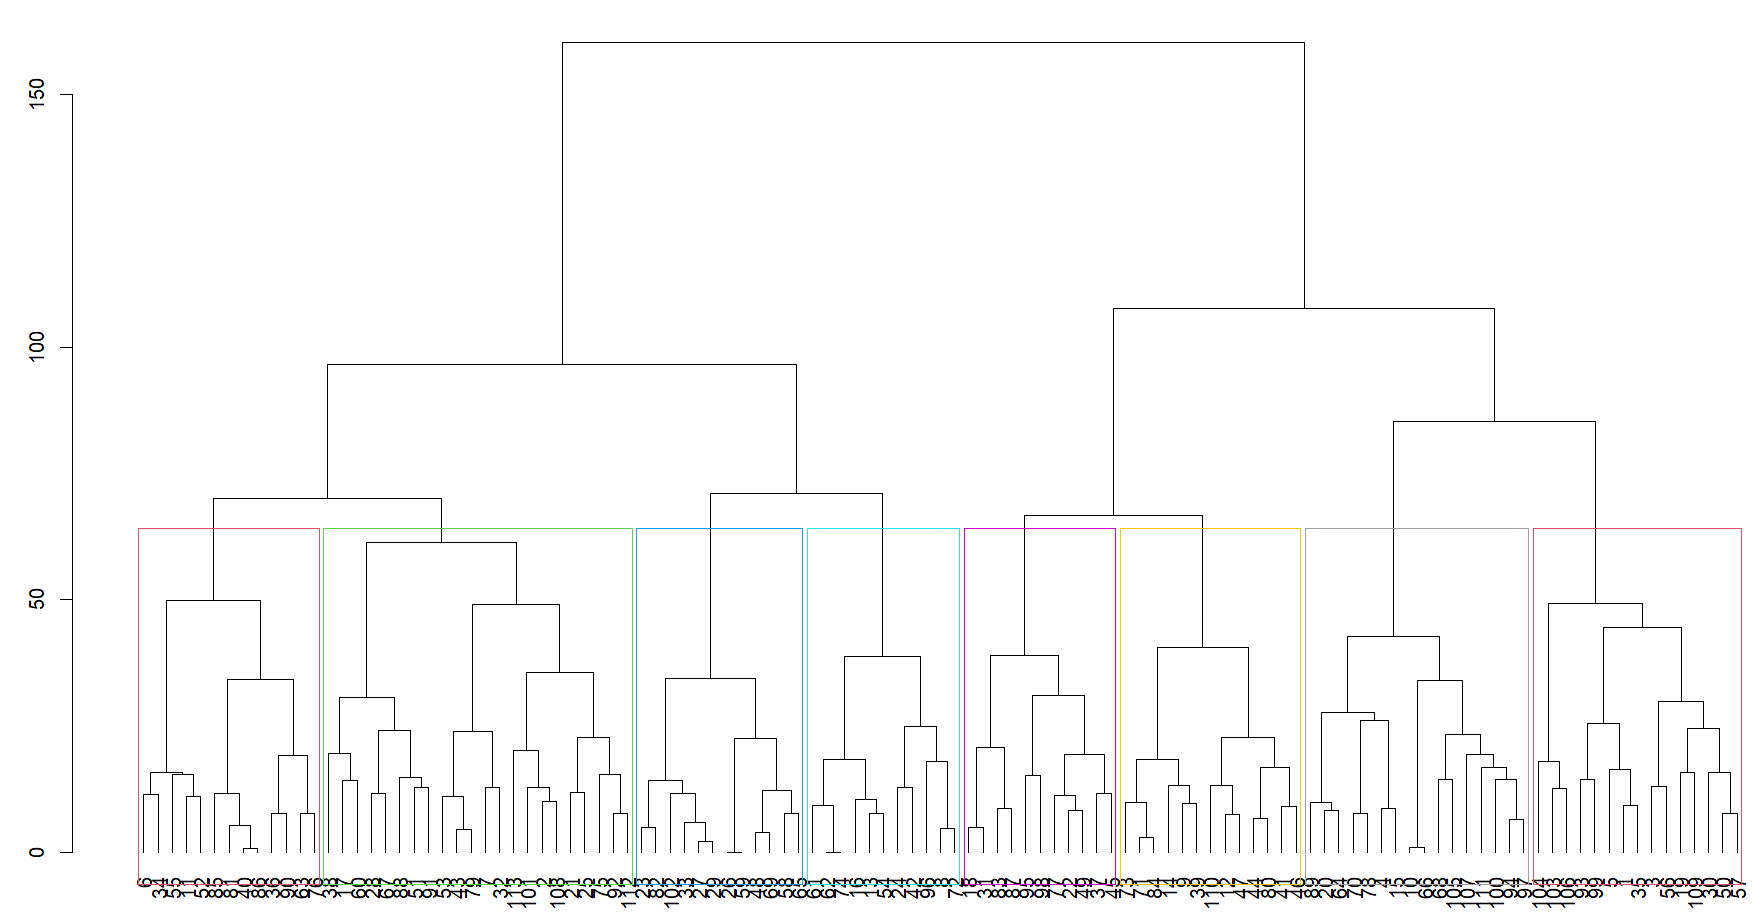
\includegraphics[scale=0.4]{graphics/dummy/dendrogram/dendrogram2.png}
        \caption{Age Distribution in each cluster}
    \end{figure}


    \subsubsection{Histogram and observing patterns}
 "Age", "Genre", "Field", "Frequency", and "Factor" are considered the main attributes of the movie genre recommender system, then we observe the patterns of those attributes by histograms.

 R code to plot the histograms for each cluster:
 \begin{code}{R}
    # Add the cluster assignments to the data frame
    df$Cluster <- factor(clusters)

    # Create a histogram of the Genre distribution in each cluster
    ggplot(df, aes(x = Genre)) +
      geom_histogram(stat = "count", fill = "lightblue", color = "black", linewidth = 0.8) +
      facet_wrap(~ Cluster) +
      theme(axis.text.x = element_text(angle = 45, hjust = 1)) +
      labs(title = "Genre Distribution in Each Cluster", x = "Genre", y = "Count")
    
    # Create a histogram of the Age distribution in each cluster
    ggplot(df, aes(x = Age)) +
      geom_histogram(stat = "count", fill = "orange", color = "black", linewidth = 0.8) +
      facet_wrap(~ Cluster) +
      theme(axis.text.x = element_text(angle = 45, hjust = 1)) +
      labs(title = "Age Distribution in Each Cluster", x = "Age", y = "Count")
    
    # Create a histogram of the Field distribution in each cluster
    ggplot(df, aes(x = Field)) +
      geom_histogram(stat = "count", fill = "red", color = "black", linewidth = 0.8) +
      facet_wrap(~ Cluster) +
      theme(axis.text.x = element_text(angle = 45, hjust = 1)) +
      labs(title = "Field Distribution in Each Cluster", x = "Field", y = "Count")
    
    # Create a histogram of the Frequency distribution in each cluster
    ggplot(df, aes(x = Frequency)) +
      geom_histogram(stat = "count", fill = "darkgrey", color = "black", linewidth = 0.8) +
      facet_wrap(~ Cluster) +
      theme(axis.text.x = element_text(angle = 45, hjust = 1)) +
      labs(title = "Frequency Distribution in Each Cluster", x = "Frequency", y = "Count")
    
    # Create a histogram of the Factor distribution in each cluster
    ggplot(df, aes(x = Factor)) +
      geom_histogram(stat = "count", fill = "lightgreen", color = "black", linewidth = 0.8) +
      facet_wrap(~ Cluster) +
      theme(axis.text.x = element_text(angle = 45, hjust = 1)) +
      labs(title = "Factor Distribution in Each Cluster", x = "Factor", y = "Count")
 \end{code}

    \begin{figure}[H]
        \centering
        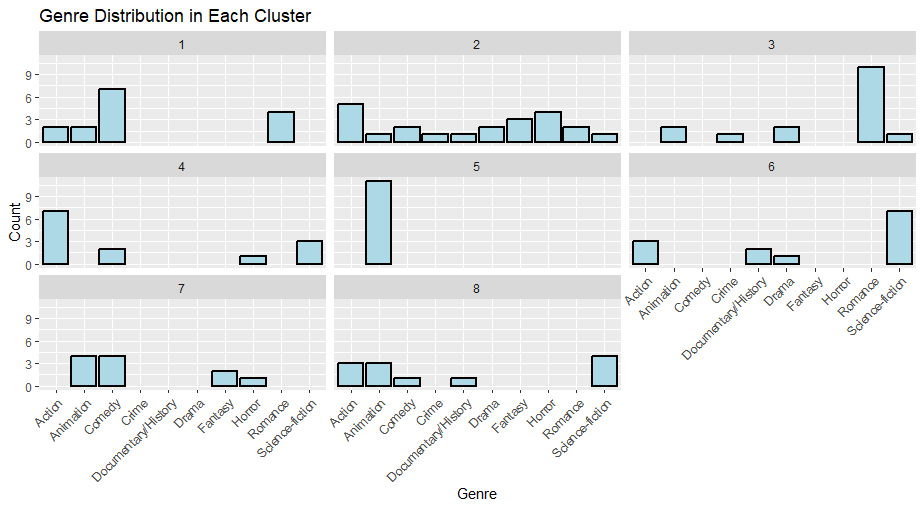
\includegraphics[scale=0.55]{graphics/dummy/distribution/GenreDistribution.png}
        \caption{Genre Distribution in each cluster}
    \end{figure}

    \begin{figure}[H]
        \centering
        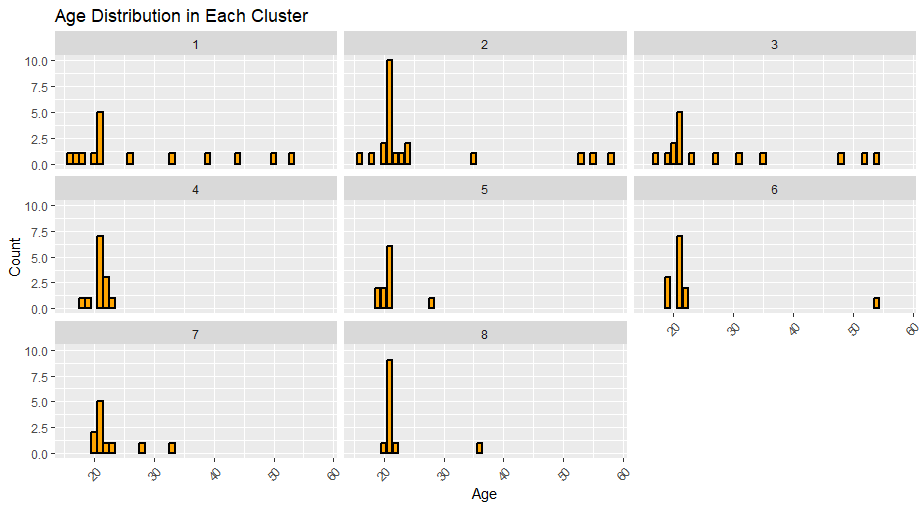
\includegraphics[scale=0.6]{graphics/dummy/distribution/AgeDistribution.png}
        \caption{Age Distribution in each cluster}
    \end{figure}

    \begin{figure}[H]
        \centering
        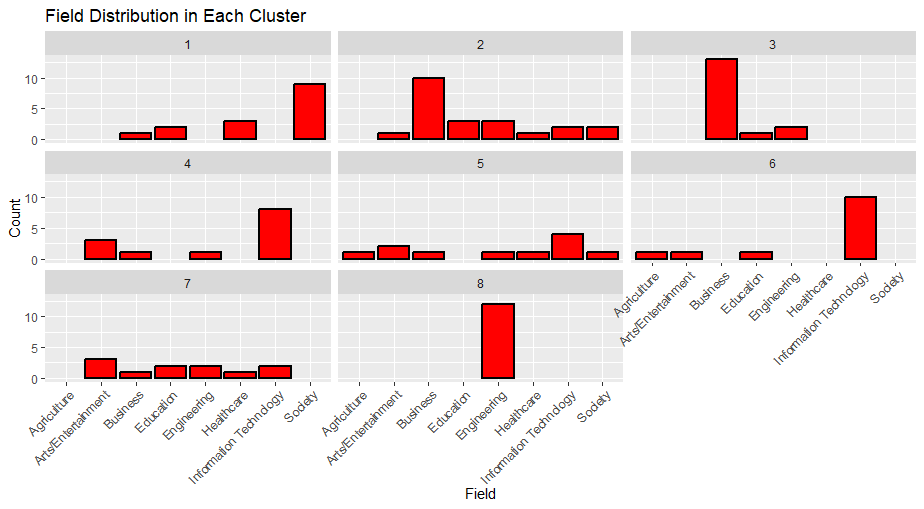
\includegraphics[scale=0.6]{graphics/dummy/distribution/FieldDistribution.png}
        \caption{Field Distribution in each cluster}
    \end{figure}

    \begin{figure}[H]
        \centering
        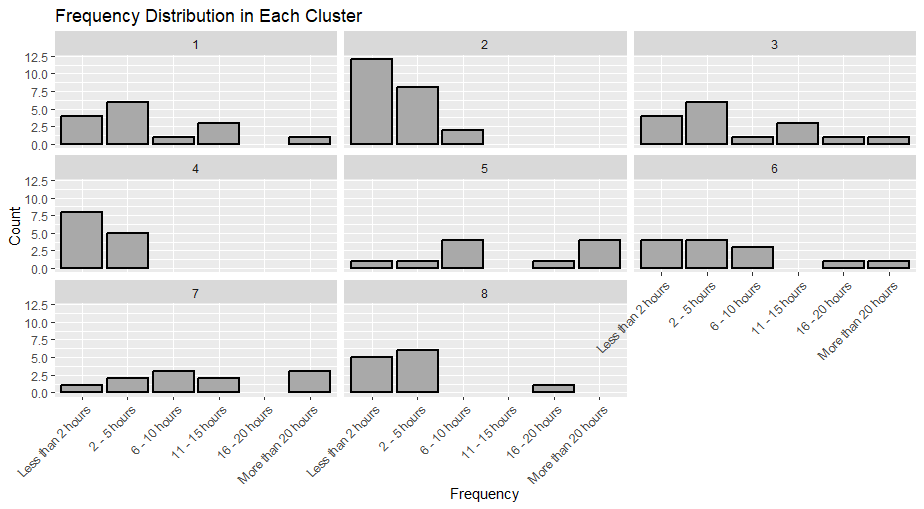
\includegraphics[scale=0.6]{graphics/dummy/distribution/FrequencyDistribution.png}
        \caption{Frequency Distribution in each cluster}
    \end{figure}

    \begin{figure}[H]
        \centering
        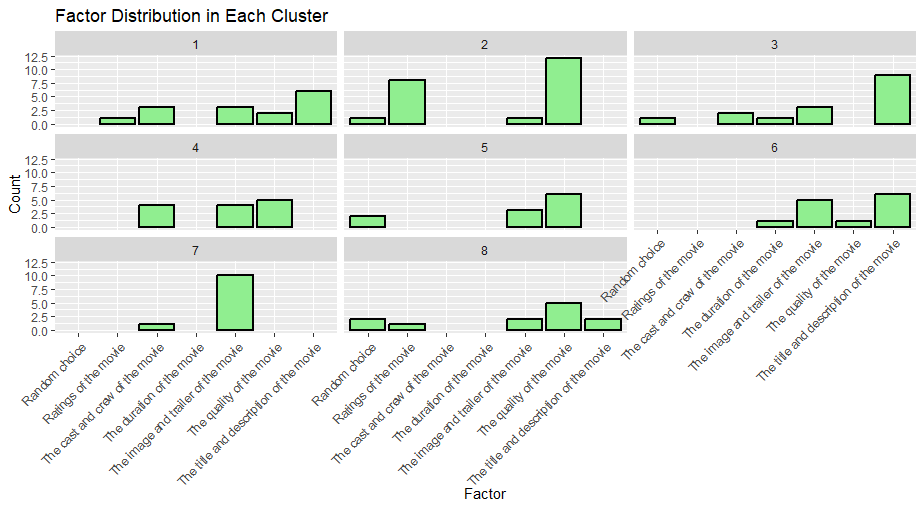
\includegraphics[scale=0.6]{graphics/dummy/distribution/FactorDistribution.png}
        \caption{Factor Distribution in each cluster}
    \end{figure}

From the histograms, here are conclusions for each cluster:

\begin{itemize}
    \item \textbf{\underline{Cluster 1:}} \textbf{Comedy} is the most favorite genre followed by \textbf{Romance}, with the majority of viewers being 21 years old and a small number ranged from 22 to 55 years old. Watching time is from 2 to 5 hours per week. Society field is the highest choice here. “Title/Description” is the most popular reason for choosing and watching.

    \item \textbf{\underline{Cluster 2:}} \textbf{Action}, \textbf{Horror}, and \textbf{Fantasy} are top-viewed genres (Romance and Drama are also considered). The viewers are mostly under 25 years old. The average watching time falls between “Less than 2 hours” and “2 - 5 hours” per week. The number is largely come from Business and evenly distributed in the Education and Engineering fields. “Ratings” and “Quality” are the two most important factors for picking movies.

    \item \textbf{\underline{Cluster 3:}} \textbf{Romance} is the top-most choice of movie genre in this cluster. The viewers are divided into 2 main age groups: around 25 and above 45 years old. Watching times are “2 - 5 hours” and “11 - 15 hours”. Business is the highest-picked field. “Title/Descriptions” is the most important factor.


    \item \textbf{\underline{Cluster 4:}} \textbf{Action} and Science-fiction are the most favorite genre, with the majority of viewers being under 21 years old. Watching time is “Less than 5 hours” per week. IT field is the highest choice here, followed by Arts/Entertainment. “Cast/Crew”, “Image/Trailer”, and “Quality” are the most popular reasons for choosing and watching.

    \item \textbf{\underline{Cluster 5:}} It is clearly seen that \textbf{Animation} is the only choice of movie genre in this cluster. The viewers are mostly 19 - 21 years old, and a small number is from 26 - 27 years old. The average watching time is pretty high and falls between “6 - 11 hours” and “More than 20 hours” per week. The number is largely come from IT and evenly distributed in the Agriculture, Arts/Entertainment, Business, Engineering, Healthcare, and Society fields. “Image/Trailer” and "Quality" are the two most important factors for picking movies.

    \item \textbf{\underline{Cluster 6:}} \textbf{Action} and \textbf{Science-fiction} are the top-most choices of movie genres. Viewers are mostly around 20 and a small one is above 50 years old. Watching time is total less than 10 hours per week. IT is the highest-picked field. “Image/Trailer” and “Title/Descriptions” are the most important factor. 

    \item \textbf{\underline{Cluster 7:}} \textbf{Animation} along with \textbf{Comedy} is the most favorite genre followed by \textbf{Fantasy} and \textbf{Horror}, with the majority of viewers being under 35 years old. Watching time varies from less than 15 hours and more than 20 hours per week. The agriculture field is the highest choice here, and there exists evenly distribution of Education, Engineering, and IT fields. “Image/Trailer” is the most popular reason for choosing and watching.

    \item \textbf{\underline{Cluster 8:}} \textbf{Action}, \textbf{Animation}, and \textbf{Science-fiction} are top-viewed genres. Viewers are mostly under 25 years old. The average watching time falls between “Less than 2 hours” and “2 - 5 hours” per week. The number is all come from Engineering fields. “Quality” and “Title/Description” are the two most important factors for picking movies.
\end{itemize}

\subsection{Advantages and Disadvantages: Dummy variables}

    \subsubsection{Advantages}

        \begin{itemize}
            \item \textbf{Nominal Data Handling:} Hierarchical clustering algorithms typically work with numerical distances or similarities between data points. Dummy variables allow us to represent nominal variables numerically, enabling their incorporation into the clustering process.

            \item \textbf{Information Preservation:} Dummy variables can help preserve information about the nature of the data. By creating separate binary variables for different categories, we maintain the distinctions between nominal variables during clustering.
        \end{itemize}


    \subsubsection{Disadvantages}
        \begin{itemize}
            \item \textbf{Unequal Distances}: Dummy variables assume equal distances between points, which might not reflect the actual dissimilarities between them. 
            
            \item \textbf{Increased Noise:} If the nominal variable has a large number of attributes with limited observations in each attribute, the dummy variables may introduce noise into the clustering process, leading to less reliable results.
        \end{itemize}
\section{Hierarchical clustering with mixed-type variables }

\subsection{Problem}
One important aspect of processing information is to deal with different types of data, because not every attribute is of the same nature. 

Given an example: A survey is conducted about a person’s daily life. The considered factors are: Age, Gender, Job, and how Satisfactory they are. A quick observation shows that these values are not the same type. Age is measured in integer, which is a numerical value; Gender can be used as a binary value, with 0 (false) being female, and 1 (true) being male; Job is shown with many options (engineer, businessman, storekeeper, homemaker, …), therefore it is a nominal value; and a scale of 1 to 10 to rate the person’s satisfaction, which is an ordinal value. This is just some common types of data that we usually deal with, so knowing how to process mixed data can benefit us with a more realistic model.

This section will discuss Gower’s Distance, which is one of the methods to deal with this problem. 

\subsection{Gower's Distance}
Gower’s Distance is a method for computing distances between two data points. The strength of this method comes from the fact that it is usable for other types of data beside numerical, which is more flexible than the common methods (Euclidean distance, Manhattan distance, …). Another advantage is that Gower’s Distance scales the ranges of data into between 0 and 1, with addition of allowing a user-defined weighting scheme. But for this project, an unweighted model is constructed. 

The basic calculation of Gower’s Distance is as follow. Data will be separated into two types: numerical and non-numerical.

With numerical, we can compute the data by the formular: 

    \quad |Difference| / Range

    \begin{itemize}
        \item Difference = Data[i] - Data[i+1] ; 
        \item Range is the difference between the maximum and the minimum data points. 
    \end{itemize}

With non-numerical values, we can compute by compare the data points. If they are identical, the distance will be 0, if not then the distance will be 1.

There are some packages that uses or have the option for Gower’s calculation, and in this project "cluster" package is used, which contains function "daisy" that allows Gower as an option.

\subsection{Code Explaination}
(Source code link: \url{https://github.com/vhtuananh020402/Group4_Data_analysis/blob/main/completed_gower_ward.r})

\vspace{1mm}
First, libraries and data frame will be imported. The function na.omit(df) is necessary for omitting missing values in the data frame.
    \begin{code}{R}
        library(factoextra)   # clustering visualization
        library(ggplot2)      # draw distribution graph

        # read data frame
        df <- read.csv("data/clean_data_v2.csv")
        # remove missing values in data frame
        df <- na.omit(df)
    \end{code}
Then, data will be processed by splitting into 3 types: numerical, nominal, and ordinal. Nominal is defined by using function lapply(df[nom\textunderscore attr], as.factor) to change value type into factor. Ordinal is defined by using function factor(), which has the option order = TRUE, and level is from lowest to highest. Finally, process\textunderscore dataset will contain the complete dataset for analysing steps.
    \begin{code}{R}
            # --- Data Preparation --- #
        # add into numerical value
        num_attr <- c("Age")

        # add into nominal value
        nom_attr <- c("Field", "Genre", "Factor")
        df[cat_attr] <- lapply(df[cat_attr], as.factor)

        # add into ordinal value
        ord_attr <- c("Frequency")
        df$Frequency <- factor(df$Frequency, 
                                    order = TRUE, 
                                    level = c("Less than 2 hours", 
                                                "2 - 5 hours", 
                                                "6 - 10 hours", 
                                                "11 - 15 hours", 
                                                "16 - 20 hours", 
                                                "More than 20 hours"))

        # put everything into a complete data set
        process_dataset <- df %>% select(num_attr, ord_attr, cat_attr)

        head(process_dataset)
    \end{code}
Function daisy() will calculate the dissimilarity matrix, with process\textunderscore dataset as input, and gower  is used as the calculation metric. After that, the hierarchical clustering model is built using hclust() function. Clustering method ward.D is chosen because it brings the best result when plotting dendrogram.
    \begin{code}{R}
            # --- Calculation --- #
        # calculate Gower's distance
        gower_dist <- daisy(process_dataset, metric="gower")   

        # hierarchical clustering, using ward.D method 
        gower_hcl <- hclust(gower_dist, method = "ward.D")  

            # --- DENDROGRAM ---- #
        # plot dendrogram
        plot(gower_hcl, cex = 0.6)

        # draw borders for the individual clusters
        rect.hclust(gower_hcl, k = 7, border = 2:7)
    \end{code}
Histograms are used to present the distribution of each attribute in each cluster. “k” represents the number of clusters that we want. The decision k = 7 is made according to the previous method of building hierarchical clustering using Dummy Variable. For some unknown reasons, the functions that find the optimal number of clusters is unusable in this section.
    \begin{code}{R}
            # --- HISTOGRAM --- #
        # cut into k clusters
        k <- 7
        clusters <- cutree(gower_hcl, k)

        # add the cluster assignments to the data frame
        df\$Cluster <- factor(clusters)

        # histogram of Genre distribution in each cluster
        ggplot(df, aes(x = Genre)) +
            geom_histogram(stat = "count", fill = "lightblue", color = "black", linewidth = 0.8) +
            facet_wrap(~ Cluster) +
            theme(axis.text.x = element_text(angle = 45, hjust = 1)) +
            labs(title = "Genre Distribution in Each Cluster", x = "Genre", y = "Count")

        # histogram of Field distribution in each cluster
        ggplot(df, aes(x = Field)) +
            geom_histogram(stat = "count", fill = "red", color = "black", linewidth = 0.8) +
            facet_wrap(~ Cluster) +
            theme(axis.text.x = element_text(angle = 45, hjust = 1)) +
            labs(title = "Field Distribution in Each Cluster", x = "Field", y = "Count")

        # histogram of Factor distribution in each cluster
        ggplot(df, aes(x = Factor)) +
            geom_histogram(stat = "count", fill = "lightgreen", color = "black", linewidth = 0.8) +
            facet_wrap(~ Cluster) +
            theme(axis.text.x = element_text(angle = 45, hjust = 1)) +
            labs(title = "Factor Distribution in Each Cluster", x = "Factor", y = "Count")

        # histogram of Age distribution in each cluster
        ggplot(df, aes(x = Age)) +
            geom_histogram(stat = "count", fill = "orange", color = "black", linewidth = 0.8) +
            facet_wrap(~ Cluster) +
            theme(axis.text.x = element_text(angle = 45, hjust = 1)) +
            labs(title = "Age Distribution in Each Cluster", x = "Age", y = "Count")

        # histogram of Frequency distribution in each cluster
        ggplot(df, aes(x = Frequency)) +
            geom_histogram(stat = "count", fill = "darkgrey", color = "black", linewidth = 0.8) +
            facet_wrap(~ Cluster) +
            theme(axis.text.x = element_text(angle = 45, hjust = 1)) +
            labs(title = "Frequency Distribution in Each Cluster", x = "Frequency", y = "Count")
    \end{code}

\subsection{Results}
    \subsubsection{Dendrogram}
        The dendrogram shows the relations between all of the observations, with each cluster is shown by colored lines. With many tries and many different methods, we decided to keep this result because this is more evenly distributed model than other versions.
        \begin{figure}[H]
            \centering
            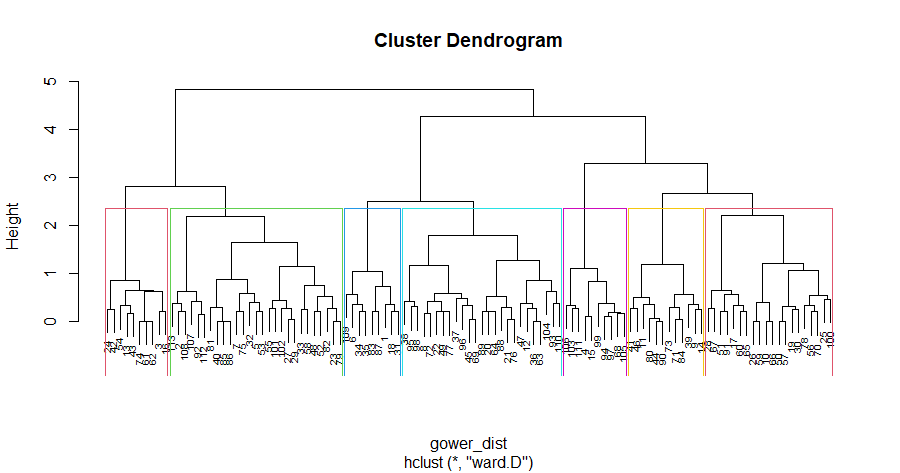
\includegraphics[scale=0.6]{graphics/gower/dendrogram/gower_dist_ward.png}
            \caption{Result visualized by Dendrogram}
        \end{figure}
    \subsubsection{Histograms and observing patterns}
        We only obverse the histograms of the following attributes: Age, Genre, Field, Frequency and Factor. Gender and Platform are useful for unifying the dataset, but those are not considered to be the attribute that contributing to the recommended system in real-world practices. Therefore, we omit them when graphing the histograms.
        \begin{figure}[H]
            \centering
            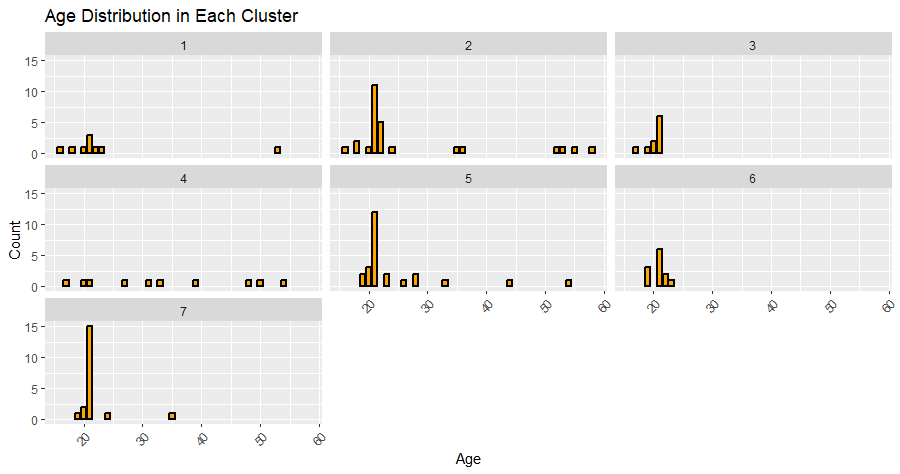
\includegraphics[scale=0.6]{graphics/gower/histogram/age distrib.png}
            \caption{Age distribution in each cluster visualized by Histogram}
        \end{figure}
        \begin{figure}[H]
            \centering
            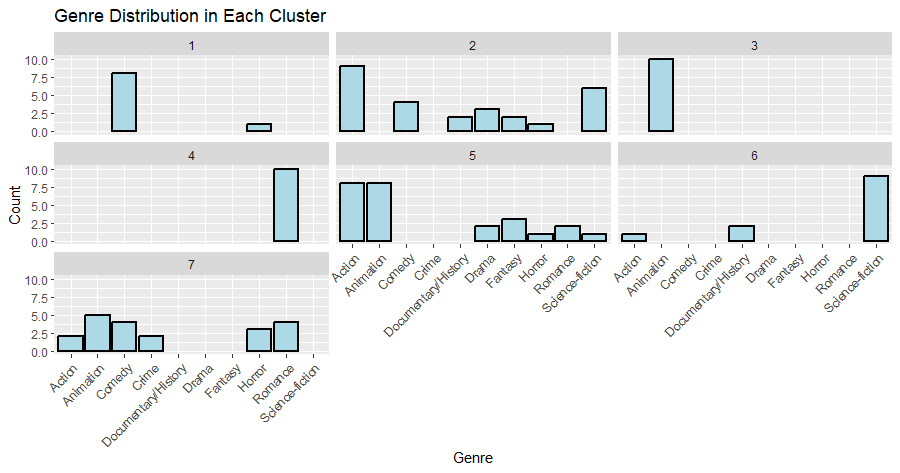
\includegraphics[scale=0.6]{graphics/gower/histogram/genre distrib.png}
            \caption{Genre distribution in each cluster visualized by Histogram}
        \end{figure}
        \begin{figure}[H]
            \centering
            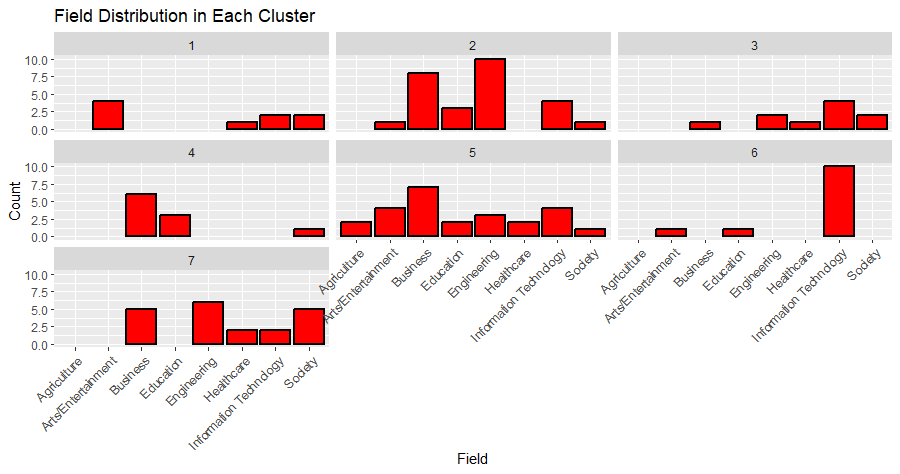
\includegraphics[scale=0.6]{graphics/gower/histogram/field distrib.png}
            \caption{Field distribution in each cluster visualized by Histogram}
        \end{figure}
        \begin{figure}[H]
            \centering
            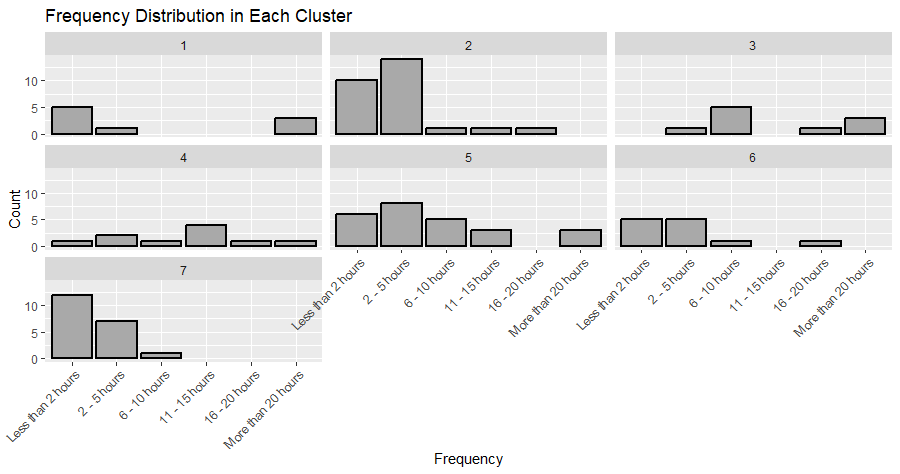
\includegraphics[scale=0.6]{graphics/gower/histogram/freq distrib.png}
            \caption{Frequency distribution in each cluster visualized by Histogram}
        \end{figure}
        \begin{figure}[H]
            \centering
            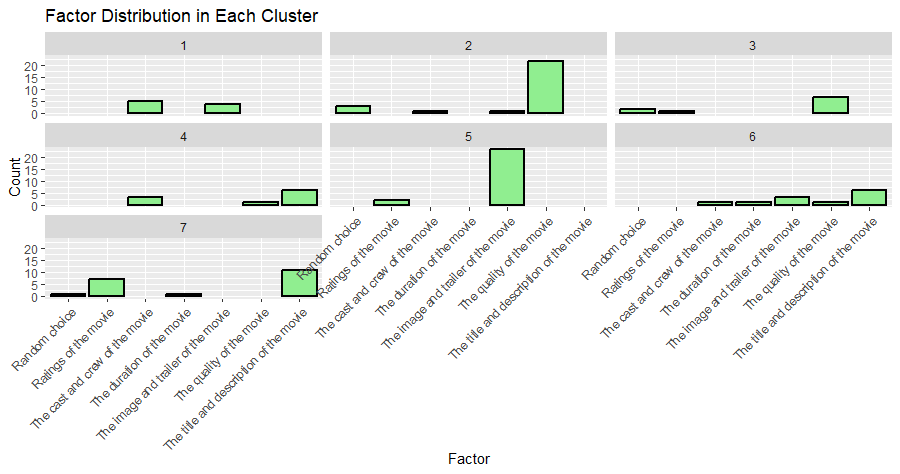
\includegraphics[scale=0.6]{graphics/gower/histogram/factor distrib.png}
            \caption{Factor distribution in each cluster visualized by Histogram}
        \end{figure}
The followings are concluded from the histogram for each cluster:
\newline

Cluster 1: Mostly from under 25 years old. Comedy is the most watched genre, with watching time falls between “Less than 2 hours” and “Over 20 hours”. Art/Entertainment field being the highest choice here, with IT and Society being the lesser. “Cast/Crew” and “Image/Trailer” are the reasons for choosing and watching.
\newline

Cluster 2: The majority are 21 years old, with Action and Sci-fi are the most viewed. Comedy, Documentary/History, Drama, Fantasy and Horror are also considered. Watching time is from 2 to 5 hours. They are largely come from Engineering and Business. “Quality” is the most important factor for picking movies.
\newline

Cluster 3: The majority are 21 years old, with Animation being the only choice for genre. “6 - 10 hours” and “more than 20 hours” are the standout choices. Engineering, IT and Society are evenly distributed fields, with IT being the highest choice. “Quality” is the most important factor.
\newline

Cluster 4: Ages are evenly distributed across the range. Romance is the only viewed genre here. Watching time is variety, with “11 – 15 hours” being the highest choice. Business is the most picked field here, and they consider “Cast/Crew” and “Title/Description” when choosing movies.
\newline

Cluster 5: Mostly 21 years old, with Action and Animation are the highest viewed genre here, also with somewhat evenly distributed between Drama, Fantasy, Romance. Watching time is largely from “Less than 2 hours” to “6 – 10 hours” range. Business is the most choice for field, but the occupation is distributed across the range. “Image/Trailer” is the most important factor.
\newline

Cluster 6: Around 20 years of age. Science-fiction is the most viewed genre, with small percentage comes from Action and Documentary/History. Mostly from “Less than 2 hours” to “2 - 5 hours” range of watching time. IT field is the highest choice, with “Image/Trailer” and “Title/Description” are the most important factor. 
\newline

Cluster 7: The majority are 21 to 22 years old. Action, Animation, Comedy, Crime, Horror and Romance shared the genre distribution without much differences. Watching periods mostly come from “Less than 2 hours” to “2 – 5 hours” range. Business, Engineering and Society are the most choices for field of occupation, and “ratings” as well as “title/description” are the most important factors.

\subsection{Shortcomings}
With the lack of documentation, using libraries that implement Gower’s Distance is complicated and troublesome, as it leads to unexpected errors. One example is that functions to find the optimal number of clusters cannot be applied, whether it is Elbow, Silhouette or Gap Statistic method. Because of the limited time frame of this project, the errors cannot be solved yet. Therefore, it is crucial to research thoroughly beforehand if using the existing libraries for this method.
\section{Conclusion}

    \subsection{Accomplishment of Project Objectives}
     %  \item We would like to group together users with similar viewing patterns in order to recommend similar content (genres). By asking different questions about age, genre, and hobbies, we can collect data and conclude some insights.
    From conducting the survey, preparing data, analyzing input, to visualizing attributes by histograms, our team can identify the relation between viewing patterns(age, film genre, working field, frequency, factor) and we can recommend content based on that insight. For that reason, our team has achieved our project goals and objectives.
    
    \subsection{Future Work}
    Refining clustering algorithms, adding more features, or expanding the recommendation system's capabilities are admirable improvements for this project. Other potential areas can be building the movie recommendation web app, testing our recommendation, accuracy; as well as implementing other methods to analyze data such as non-hierarchical clustering, and comparing the result between two methods. 



    

% citation - references
\bibliographystyle{plainurl}
\bibliographystyle{plain}
\bibliography{refs.bib}
\nocite{*}

\end{document}
